\documentclass{article}
\usepackage{graphicx}
\begin{document}

%-------------------------------------------------------------------------------
%    TITLE PAGE
%-------------------------------------------------------------------------------

\begin{titlepage}
\newcommand{\HRule}{\rule{\linewidth}{0.5mm}}
\center
\textsc{\LARGE Imperial College London}  \\[1.5cm]
\textsc{\Large Department of Computing}  \\[0.5cm]
\textsc{\large Course 350: Management and Business for Computing Engineers} \\[0.5cm]

\HRule \\[0.6cm]
{\huge \bfseries name of company here} \\[0.3cm]
\HRule \\[1.5cm]

\begin{minipage}{0.4\textwidth}

% author
\begin{flushleft} \large \emph{Authors:} \\
Alina     \textsc{Boghiu}    \\
Giovanni  \textsc{Charles}   \\
Adam      \textsc{Fiksen}    \\
Sahil     \textsc{Jain}      \\
\L ukasz  \textsc{Koprowski} \\
Rutwik    \textsc{Shah}      \\
John      \textsc{Walker}    \\
\end{flushleft}

% supervisors
\end{minipage}~
\begin{minipage}{0.4\textwidth}

\begin{flushright} \large \emph{Lecturer:} \\
Nick \textsc{Coutts}
\end{flushright}


\end{minipage}\\[4cm]

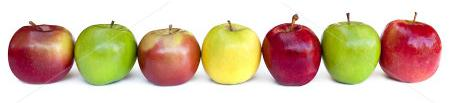
\includegraphics[width=\textwidth]{apples.jpg}

\end{titlepage}

%-------------------------------------------------------------------------------

\section{Executive summary}

business model = product (disguised as service for legal reasons - absolut?)

business objective 
maximise sales 
 - new to the market
   explain the required infrastructure to sell a lot 

\section{Vision statement}

Our mission is to bring a mid priced cider to the people of India. India
has the second largest population in the world, and has an estimated market size
of 500 million alcohol consumers [better estimate]. At the moment, there is one 
provider of cider in India, and we would like the change that.

We want to be a brewery. We will brew our own cider in the state of Himachal
Pradesh, which is the source of the majority of the apples in India. Along with
producing cider, we will sponsor other exclusive bars and clubs.

Operating in India which is well known for its corruption, we want to practice
ethical development. eg corrupt free, no bribes, no blood cider forced labour
fairtrade

We hope to gain popularity in major establishments, in Delhi and Mumbai through 
the open minded youth and bar owners.

Our cider will become a desired commodity through exclusivity and we will be
able to research our market further at this point with minimal risk.

We will adapt and pick up popularity and scale up to make it available to the
public. 

%please discuss even if you do not think it is an issue
Operating in India which is well known for its corruption, we want to practice
ethical development. eg corrupt free, no bribes, no blood cider forced labour
fairtrade

ethics.
fairtrade - look at poverty + with partners
poverty - provide jobs and food to the villagers. improve infrastructure (added benefits - tax exemptions) 
religion - no issue, alcohol is still sold across all of india 
corruption - no bribes, do everything by the books 
age restriction - different restrictions for different states, alcohol content 
health - people already drink, we arent trying to get more people to drink, just introduce it to current drinkers
eco(water recycling, using up all the apples) - recycle apple waste. recycle all water. solar energy. supply of apples
%add as you please

type = pvt. ltd. co. - control of the company

\section{Management team}

\section{Introduction to the market}
\section{Products and services offered}
\section{Marketing plan}

there is only one other provider of this product hence we see very low competition in this field 

Introducing to bars, clubs and hotels in the major cities in India (Delhi, Mumbai, Goa,
Bangalore, Kolkata). Each city would give a different version of the cider, so we would
get a general idea of what the market prefers taste wise.

Low calorie cider?

Need to make other items with the saame brand name, because advertising is limited. Surrogate advertisement

Affiation with a charity? Provide consumers a "feel good" feeling while buying alcohol.

Corruption free

Use of TV and radio. around a billion people listen to the radio, so sponsor the primetime radio
show to spread the name.

Affiliation with the IPL. International market, so easy to introduce Indians to cider.

Cost based pricing vs Price based costing. Cant do competitive analysis, as no cider exists, but compete with
the local beers, etc. Price based costing wins btw.


 % summary of detailed plan including
	% prioritisation
	% validation
	% offers
	% routes to market

objective - maximise sales -> how

LTV = (Tn + ATV + LT) - (CoA + CoR) 
options which affect LTV

tailor LTV to get maximise value for target customer - guesswork market research
needs to be conducted

how this affects the supply chain
\section{Revenue model}
\section{Resource, cost and implementation plan}
revenue
 - retail
   licence
   other sales

profit
 - gross
   net
   EBITDA
   NPV

costs
 ...

sources of capital
 % Including headcount plan
\section{Product and systems development plans}
In order to setup a stable and longlasting infrastructure for our business we must take into consideration all the stages and requirements of production. This outlines a coherent development plan as follows.

	\begin{enumerate}
	\item Factory \\
When deciding about our homebase we considered two main criteria. The first regards our situation as a new company without assets. This brought the decision of renting out the factory bulding and equipment. The second criteria regards our main ingrediant requirements. Apples in India are available in the region of Himachal Pradesh. \\

For these reasons we will set our factory near Shimla, capital of Himachal Pradesh and rent the space and equipment necessary for production \\

\textbf{Quantities and Workforce} \\
For our marketing plan we require a relatively small production volume.\\
Workforce availability. \\

\textbf{Quality control}
We must ensure a good quality especially because it is a new product for this market..

	\item Suppliers
		\begin{itemize}
		\item Apple supply \\
			Buy from local farmers %who?
        	Sell residue back to farmers for animals (or agree on lower price)
		\item (Potentially) mango, berries, pares etc. suppliers
		\item Water supply \\
			Divine Waters, Foods Beverages
		\item Sugar supply %who?
		\item Bottling \\
			Home brewers use beer bottles, which work perfectly well, and are inexpensive. This allows the cider to become naturally carbonated.
		\end{itemize}
			
\item Risks \\
Eliminated some risk by:\\
	renting instead of building the factory\\
	buying instead of growing own apples\\
Workforce: lack of experience\\
Collaborators: \\
	\end{enumerate}


%1. how much money do we have
%2. how much can we do without partners
%3. where do we setup factories
%	what gets done in the factory
%4. where do we purchase equipment from
%5. who do we need to work for us
%6. distribution (how?)

\section{Capital requirements}
\section{Business opportunities and risks}
\section{Pro-forma financial projections}
\section{Risk analysis}

\end{document}
